% !TEX root = ../../Build/main.tex
% ###################################################################
% Copyright (c) 2025, M. De Graef 
%  Editors: A.D. Rollett & M. De Graef
% All rights reserved.
%
% Licensed under the Creative Commons CC BY-NC-SA 4.0 License, 
% hereafter referred to as the "License"; you may not use this 
% document except in compliance with the License. You may obtain 
% a copy of the License at 
%     https://creativecommons.org/licenses/by-nc-sa/4.0/legalcode 
% Unless required by applicable law or agreed to in writing, all 
% material distributed under the License is distributed on an 
% "AS IS" BASIS, WITHOUT WARRANTIES OR CONDITIONS OF ANY KIND, 
% either express or implied. See the License for the specific 
% language governing permissions and limitations under the License.
% ###################################################################

% ###################################################################
% The following lines are to be uncommented or edited as needed 

\corechapter{Yes}
%     uncomment this line only if this chapter is a core/foundational chapter;
%     for a core chapter a "Core" label will appear on the top left above the chapter title.

\OCchapterauthor{Marc De Graef, Carnegie Mellon University}
%     this will appear in a secondary header below the chapter title.

% All figures are stored in the src/Tensors/eps folder and must be of the *.eps type. 
\renewcommand{\chaptergraphicspath}{../src/Tensors/eps/}

% this is the 6-character (all uppercase) chapter descriptor used in labels and refs...
\renewcommand{\chabbr}{TENSOR}

%     replace \noheaderimage by the chapter header image file name (without .eps extension).
%     Chapter header images must be 2480 x 1240 pixels with 300dpi, RGB format.
\chapterimage{\noheaderimage}

% start the chapter and define the chapter label (outside of the \chapter command!)
\chapter{Introduction to Tensors}\OClabel{Tensors}

% add the author information so that it will appear in the Author List at the start of the document
\writeauthor{TENSOR:Tensors}{Introduction to Tensors}{De Graef}{Marc}{Materials Science and Engineering}{Carnegie Mellon University}{mdg@andrew.cmu.edu}{https://www.mse.engineering.cmu.edu/directory/bios/degraef-marc.html}

% Each chapter begins with Learning Objectives; the list of objectives should have links to sections/subsections using their OC labels
% each Learning Objective should be an active statement (i.e., contain a verb).  The \\ command can be used to force an item into the 
% second column if LaTeX breaks the line at an awkward location.
\lightgraybox{\begin{center}
    {\LARGE\sffamily\bfseries {\color{OCBurntOrange}\textbf{Learning Objectives}}}\\[1em]
\end{center}

{\color{OCalmostblack}\sffamily
\begin{multicols}{2}
\begin{itemize}
    \item[{\color{OCBurntOrange}\OCref{vectorproduct}:}] Discover a new product between two or more vectors
    \item[{\color{OCBurntOrange}\OCref{tensorproducts}:}] Learn the ways tensors can be multiplied (subscript rules)
    \item[{\color{OCBurntOrange}\OCref{tensortrafo}:}] Determine how tensors behave under coordinate transformations
%    \item[{\color{OCBurntOrange}\OCref{algebras}:}] Learn about Normed Division Algebras
%    \item[{\color{OCBurntOrange}\OCref{othernumbers}:}] Discover other number systems, such as dual numbers and split numbers
\end{itemize}
\end{multicols}}}
% ###################################################################
% ###################################################################
% ###################################################################


% ###################################################################

\section{A new Vector Product}\OClabel{vectorproduct}

\subsection{Products we already Know}\OClabel{knownproducts}
In most vector calculus courses, two types of products between vectors are introduced: the \indexit{scalar product} or \indexit{dot product} and the \indexit{vector cross product}.  Each of them can be defined in a geometric way as well as an algebraic way:
\begin{itemize}
	\item \textbf{\textit{dot product}}: Consider two vectors $\mathbf{p}$ and $\mathbf{q}$ with real components $p_i$ and $q_j$ with respect to a Cartesian reference frame with basis vectors $\mathbf{e}_i$, so that
	\[
		\mathbf{p} = p_i\mathbf{e}_i\text{ and }\mathbf{q}=q_j\mathbf{e}_j,
	\]
	where the summation convention is adopted\footnote{A summation is implied over any index that occurs twice on the same side of an equation.}. The dot product can then be defined in two ways: geometrically we have
	\begin{equation}
		\mathbf{p}\cdot\mathbf{q} \equiv \vert\mathbf{p}\vert\,\vert\mathbf{q}\vert\,\cos\theta,
	\end{equation}
	where $\vert\,\,\,\vert$ indicates the norm of the vector and $\theta$ is the angle between the two vectors; or algebraically,
	\begin{equation}
		\mathbf{p}\cdot\mathbf{q} = (p_i\mathbf{e}_i)\cdot(q_j\mathbf{e}_j) = p_i (\mathbf{e}_i\cdot\mathbf{e}_j)q_j = p_i\delta_{ij}q_j=p_iq_i=p_xq_x+p_yq_y+\ldots
	\end{equation}
	where $\delta_{ij}$ is the identity matrix.  Note that this equation is valid in a vector space of arbitrary dimension $N$; for each additional dimension there is an additional term in the form of the product of the two corresponding vector components.  Hence, the dot product can be defined for pairs of vectors of any dimension.

	\item \textbf{\textit{cross product}}: For the cross product, one can show that it can only be defined in vector spaces of dimension $3$ or $7$;  the mathematical proof of this statement requires some very intricate mathematical reasoning far outside the scope of this chapter.\footnote{It is not possible to define the vector cross product in spaces of dimension other than $3$ or $7$ using an approach that is similar to that used in 3D; it is possible, however, to define a related product, the \indexit{wedge product}, $\mathbf{p}\wedge\mathbf{q}$, which takes on a special role in the theory of \indexit{Geometric Algebra} (GA); GA can be formulated in spaces of arbitrary dimension.}  In this chapter, we will stick to the traditional definition in 3D.  Once again, there is a geometrical definition and an algebraic one; the geometrical definition is:
	\begin{equation}
		\mathbf{p}\times\mathbf{q} \equiv \vert\mathbf{p}\vert\,\vert\mathbf{q}\vert\,\sin\theta\, \hat{e}_{pq},
	\end{equation}
	where $\hat{e}_{pq}$ is a unit vector perpendicular to both $\mathbf{p}$ and $\mathbf{q}$, as shown in Fig.~\OCref{vproducts}(b).  The direction of this unit vector with respect to the plane formed by the two vectors is determined from the \indexit{right-hand rule}, which states that if the fingers of the right hand are curled from $\mathbf{p}$ to $\mathbf{q}$ (for the product $\mathbf{p}\times\mathbf{q}$), then the thumb points in the direction of $\hat{e}_{pq}$. The length of the cross product vector corresponds to the area of the parallellogram formed by the two vectors; since the vector $\hat{e}_{pq}$ has a well defined direction, one can think of this area as a ``signed area''.  If we changed the order of the two vectors, then the unit vector would change sign, i.e., $\mathbf{p}\times\mathbf{q}=-\mathbf{q}\times\mathbf{p}$, but the absolute value of the area would not change.
	
	The algebraic form of the vector cross product requires a little more work. We start with the Cartesian expansions of the vectors and write out the explicit cross products of the basis vectors:
	\begin{equation}
		\begin{split}
			\mathbf{p}\times\mathbf{q} 	&= p_xq_x {\color{OCCarnegieRed}\mathbf{e}_x\times\mathbf{e}_x} + p_xq_y \mathbf{e}_x\times\mathbf{e}_y-p_xq_z {\color{OCblue}\mathbf{e}_z\times\mathbf{e}_x}\\
									&\quad - p_yq_x {\color{OCblue}\mathbf{e}_x\times\mathbf{e}_y} + p_yq_y {\color{OCCarnegieRed}\mathbf{e}_y\times\mathbf{e}_y}+p_yq_z \mathbf{e}_y\times\mathbf{e}_z\\
									&\quad+ p_zq_x \mathbf{e}_z\times\mathbf{e}_x - p_zq_y {\color{OCblue}\mathbf{e}_y\times\mathbf{e}_z}+p_zq_z {\color{OCCarnegieRed}\mathbf{e}_z\times\mathbf{e}_z}.
		\end{split}
	\end{equation}
	From the geometrical definition we see that the cross product of a vector with itself must vanish, i.e. $\mathbf{e}_i\times\mathbf{e}_i=0$ (no summation over $i$); those terms are highlighted in red above.  The terms in blue had their sign changed (and thus the order of the vectors), so that we can group them with the terms in black:
	\begin{equation}
		\mathbf{p}\times\mathbf{q} = (p_xq_y- p_yq_x) \mathbf{e}_x\times\mathbf{e}_y+(p_yq_z-p_zq_y) \mathbf{e}_y\times\mathbf{e}_z+(p_zq_x-p_xq_z) \mathbf{e}_z\times\mathbf{e}_x\ .
	\end{equation}
	Finally, using the fact that the Cartesian reference frame is a right-handed orthonormal reference frame we substitute the remaining cross products by the appropriate basis vector and reorder the terms to arrive at the familiar expression for the cross product:
	\begin{equation}
		\mathbf{p}\times\mathbf{q} = (p_yq_z-p_zq_y) \mathbf{e}_x+(p_zq_x-p_xq_z) \mathbf{e}_y+(p_xq_y- p_yq_x) \mathbf{e}_z\ .
	\end{equation}
	Note that this relation can also be formulated as a $3\times 3$ determinant by writing the basis vectors on the top row, and the vector components (in the correct order) on the second and third row:
	\begin{equation}
		\mathbf{p}\times\mathbf{q} = \det\deterthree{\mathbf{e}_x}{\mathbf{e}_y}{ \mathbf{e}_z}{p_x}{p_y}{p_z}{q_x}{q_y}{q_z}\ . 
	\end{equation}
	
\end{itemize}

\subsection{The Tensor Product}\OClabel{tensorproduct}
The vector dot product represents the basic step used when multiplying conformable matrices\footnote{Two matrices $A$ and $B$ are conformable if the number of columns in $A$ is the same as the number of rows in $B$.}: take row $i$ from the first matrix and compute the dot product with column $j$ from the second matrix to obtain entry $(i,j)$ of the resulting product matrix. This means that we can also write the dot product as:
\begin{equation}
	\mathbf{p}\cdot\mathbf{q} = \rowthree{p_x}{p_y}{p_z}\columnthree{q_x}{q_y}{q_z} = p_xq_x+p_yq_y+p_zq_z\ .
\end{equation}
We can consider this as a matrix product of a $1\times 3$ matrix with a $3\times 1$ matrix to obtain a $1\times 1$ matrix, i.e., a scalar. If we change the order of the product to a $3\times 1$ matrix multiplied by a $1\times 3$ matrix (note that they are indeed conformable, so this product is meaningful), then we will obtain a $3\times 3$ matrix.  Such a product is known as an \indexit{outer product} or \indexit{tensor product} and is defined as:
\begin{equation}
	\mathbf{p}\otimes\mathbf{q} = \columnthree{p_x}{p_y}{p_z}\rowthree{q_x}{q_y}{q_z}=\matrixtbtb{p_xq_x}{p_xq_y}{p_xq_z}{p_yq_x}{p_yq_y}{p_yq_z}{p_zq_x}{p_zq_y}{p_zq_z}\ .
\end{equation}
This is clearly the most general product possible between two vectors, taking one component from the first vector and one component from the second vector.  In index notation we have:
\begin{equation}
	(\mathbf{p}\otimes\mathbf{q})_{ij} = p_i\, q_j\ .
\end{equation}
Instead of writing $\mathbf{p}\otimes\mathbf{q}$ explicitly, it is common practice to replace it by a single letter symbol, say $r$, so that:
\begin{equation}
	r_{ij} = p_i\, q_j\ .
\end{equation}
The object created by this tensor product is known as a \indexit{second rank tensor}, where the word ``second'' refers to the fact it has two subscripts (i.e., it was generated by combining two vectors). This brings up the possibility of taking the tensor product of more than two vectors, for instance the three vectors $\mathbf{s}$, $\mathbf{t}$, and $\mathbf{u}$:
\begin{equation}
	(\mathbf{s}\otimes\mathbf{t}\otimes\mathbf{u})_{ijk} = s_i\,t_j\,u_k\ .
\end{equation}
Note that it is not easy to write this result as a matrix since it would be a $3\times 3\times 3$ matrix with $27$ entries. The subscript notation on the other hand allows for a very compact notation; if we represent the left hand side object by $T$, then we have $T_{ijk}=s_i\,t_j\,u_k$, and $T_{ijk}$ is known as a \indexit{third rank tensor}.  Since the rank of a tensor is equal to the number of subscripts, this means that a regular vector $\mathbf{q}$ with components $q_i$ is a rank-1 tensor, and a scalar $\alpha$, without any subscripts, can be considered to be a rank-0 tensor.

One might ask the question: so, what are these vectors that we apparently need to build a tensor?  It turns out that it really doesn't matter that much. A simple example will show why that is the case. Consider a second rank tensor in a 2D vector space, built from the vectors $\mathbf{p}=(p_x,p_y)$ and $\mathbf{q}=(q_x,q_y)$.  Their tensor product is:
\begin{equation}
	\mathbf{p}\otimes\mathbf{q} = \columntwo{p_x}{p_y}\rowtwo{q_x}{q_y}=\matrixtwob{p_xq_x}{p_xq_y}{p_yq_x}{p_yq_y}\ .
\end{equation}
If we assign specific values to the components, say $\mathbf{p}=(3,4)$ and $\mathbf{q}=(5,6)$, then we obtain the array:
\begin{equation}
	\mathbf{p}\otimes\mathbf{q} = \matrixtwob{15}{18}{20}{24}\ .
\end{equation}
Suppose that we would like to find out what the original vectors were that gave rise to this tensor product; we would then need to solve the following equations:
\begin{equation}
	\begin{split}
		p_xq_x &= 15;\\
		p_xq_y &= 18;\\
		p_yq_x &= 20;\\
		p_yq_y &= 24.
	\end{split}
\end{equation}
This system of equations does not have a unique solution; using Mathematica, we find that the solutions can only be expressed in terms of one remaining unknown, namely $p_x$. The solution for the other three components is
\begin{equation}
	\begin{split}
		p_y &= \frac{4 p_x}{3};\\
		q_x &= \frac{15}{p_x};\\
		q_y &= \frac{18}{p_x}.
	\end{split}
\end{equation}
So, while a second rank tensor is defined by a tensor product of two vectors, it is a meaningless question to  ask, given the tensor, what are the vectors?  There is an infinite family of vector pairs that will produce the same tensor product.  While the exact values of the vector components don't matter, it \textit{does} really matter that the second rank tensor is defined by a tensor product of two vectors; as we will see in section~\OCref{tensortrafo}, the tensor will \textit{inherit} the transformation rules for the individual vectors when the reference frame is changed.   Before we introduce the transformation rules for general tensors, let's first do some index gymnastics.


\section{Tensor Multiplication}\OClabel{tensorproducts}
Just like real numbers and complex numbers (see chapter~\ref{NUMSYS:NumberSystems}), tensors, which are really just arrays of numbers, can be multiplied with each other.  Let's start with a simple example: the product of two second rank tensors. Consider the tensors $\kappa_{ij}$ and $\lambda_{kl}$; we know that they are each defined by a tensor product of two vectors.  While we don't care about the components of those vectors, we can still write each tensor as a tensor product of two vectors (we'll just pick some letters to represent the vectors):
\begin{equation}
	\begin{split}
		\kappa_{ij} & = (\mathbf{a}\otimes\mathbf{b})_{ij};\\
		\lambda_{kl} & = (\mathbf{c}\otimes\mathbf{d})_{kl}.
	\end{split}
\end{equation}
Each of these tensors can be written as a $3\times 3$ matrix.  Since they are tensors, we can multiply them together using the tensor product, so we create a new quantity with four subscripts:
\begin{equation}
	\kappa_{ij}\lambda_{kl} \equiv \mu_{ijkl} =  (\mathbf{a}\otimes\mathbf{b}\otimes\mathbf{c}\otimes\mathbf{d})_{ijkl}\ .
\end{equation}
Alternatively we could express $\mu_{ijkl}$ are tensor product of the two second rank tensors as well:
\begin{equation}
	\mu_{ijkl} =  (\bm{\kappa}\otimes\bm{\lambda})_{ijkl}\ .
\end{equation}
Note that the order of the subscripts is important and should always be respected. The tensor $\mu_{ijkl}$ has four subscripts and therefore it is a fourth rank tensor; it has $3^4=81$ individual components and, in principle, it can be written out explicitly as a $3\times 3$ array of $3\times 3$ arrays\footnote{The whole point of the subscript notation is that we \textbf{don't} have to write out all the individual components; we can just represent any component by its subscripted symbol, i.e, $\mu_{xxyz}$. Besides, writing all $81$ components of $\mu_{ijkl}$ would be prone to typos and other mistakes.}.  As a rule, any object created by a tensor product, or a series of tensor products, is always a tensor of a higher rank.  The rank is given by the number of subscripts, or by one more than the number of $\otimes$ product symbols.

So far, we have seen how we can multiply two tensors of ranks $r_1$ and $r_2$ together to obtain a new tensor of rank $r_1+r_2$.  However, we need to be careful; the new tensor will only have rank $r_1+r_2$ if all the subscripts of the first tensor \textit{are different} from those of the second tensor.  Consider the following three tensors: $\kappa_{ijk}$, $\lambda_{mno}$, and $\mu_{mjk}$; here are the potential products between those tensors:
\begin{itemize}
\item $\kappa_{ijk}\lambda_{mno} = \tau_{ijkmno}$: this product produces a tensor of rank $6$ because all the indices are represented by different letters;
\item $\kappa_{ijk}\mu_{mjk} = \sigma_{im}$: the subscripts $j$ and $k$ each occur twice on the same side of the equation, so there are two implied summations, and the only remaining subscripts are $i$ and $m$.  The result of this product is a second rank tensor;
\item $\lambda_{mno}\mu_{mjk}=\omega_{nojk}$: there is one summation over $m$, so the result is a fourth rank tensor.\\
\end{itemize}

\noindent These examples lead us to formulate the following rules for tensor manipulation:
\begin{itemize}
	\item There is an implied summation over any index that occurs twice on the same side of an equation; this is known as the \indexit{summation rule}.  As an example we have $\mu_{ii}=\alpha$; we have a sum of the diagonal terms on the left hand side, and this results in a scalar (the trace of the matrix in this case) on the right hand side.  Note that the rank of the right hand side is two less than the rank on the left, because the summation causes two subscripts to disappear on the left.  In general, this is known as \indexit{tensor contraction}.
	\item The overall tensor rank must be the same on both sides of an equation (after eliminating pairs by the summation rule).  As an example, consider $\kappa_{ij}\lambda_{jk}=\sigma_{ik}$; the overall rank is two on both sides, because the summed indices do not count in the rank determination.
	\item If an index occurs on one side of an equation, it must also occur on the other side, except when it is a summation index in which case the other side can not have that same index; this is known as the \indexit{index conservation rule}.
\end{itemize}
These simple rules allow us to quickly spot invalid equations; can you see why the following relations are invalid? [answers in the footnote\footnotemark{}]
\begin{itemize}
\item (1) $\lambda_{ijk}\sigma_{klm} = \alpha_{ijm}$
\item (2) $\sigma_{ii} = \lambda_i$ 
\item (3) $c_{ijklmn}\epsilon_{kl}\epsilon_{mn} = q$
\end{itemize}

\footnotetext{\rotatebox{180}{{\parbox{\linewidth}{(1) after the summation of $k$, four subscripts remain on the left; the subscript $l$ is missing on the right hand side; (2) the summation on the left ``consumes'' the index $i$, so it cannot be present on the right; (3) the subscripts $i$ and $j$ are only present on the left; they must also be present on the right since there is no summation over them.}}}}


\newpage
\section{Tensors and Coordinate Transformations}\OClabel{tensortrafo}

\subsection{Derivation of a coordinate transformation matrix}

Let us consider two Cartesian reference frames, one given by the orthonormal triplet $\{\mathbf{e}_x,\mathbf{e}_y,\mathbf{e}_z\}$, the second by the triplet 
$\{\mathbf{e}_x^{\,\prime},\mathbf{e}_y^{\,\prime},\mathbf{e}_z^{\,\prime}\}$.  We also consider a vector, $\mathbf{q}$ with components $q_j$ with respect to the reference frame $\mathbf{e}_j$, so that $\mathbf{q}=q_j\mathbf{e}_j$.  The components $q_j$ are the projections of $\mathbf{q}$ onto each of the basis vectors $\mathbf{e}_j$ so that we can write:
\[
	\mathbf{q} = (\mathbf{q}\cdot\mathbf{e}_j) \mathbf{e}_j\ .
\]
This must be valid for every vector $\mathbf{q}$, so in particular it must be valid when we pick one of the basis vectors of the primed reference frame, say $\mathbf{q}=\mathbf{e}'_x$:
\[
	\mathbf{e}'_x = (\mathbf{e}'_x\cdot\mathbf{e}_j) \mathbf{e}_j\ .
\]
This expresses the new basis vector $\mathbf{e}'_x$ as a linear combination of all three old basis vectors $\mathbf{e}_j$ (note that there is a summation over the index $j$).
In general, we can write:
\[
	\mathbf{e}'_i = (\mathbf{e}'_i\cdot\mathbf{e}_j) \mathbf{e}_j;
\]
We can collect the nine numbers $\mathbf{e}'_i\cdot\mathbf{e}_j$ in a $3\times 3$ matrix which we will represent by $\alpha_{ij}$, with:
\[	
	\alpha_{ij} \equiv \mathbf{e}'_i\cdot\mathbf{e}_j.
\]
Therefore, we have a compact relation that expresses the new basis vectors in terms of the old ones:
\begin{equation}
	\mathbf{e}'_i = \alpha_{ij}\mathbf{e}_j.\OClabel{alphadef}
\end{equation}
This is a linear relation between two basis vector triplets and is known as a \indexit{coordinate transformation}.  We will assume throughout this text that the origin itself does not change during the coordinate transformation.  If there were a change in the position of the origin as well, then we would have to add a translation vector to the equations above.  The transformation described by the matrix $\alpha_{ij}$ is known as a 3D rotation.
 
The inverse transformation must also exist and is described by the inverse of the matrix $\alpha_{ij}$:
\begin{equation}
	\mathbf{e}_i=\alpha^{-1}_{ij}\mathbf{e}_{j}^{\,\prime}.\OClabel{basistrafoinverse}
\end{equation}
It is an important property of this type of transformation matrix that the inverse of the matrix is equal to the transpose; matrices with this property are known as orthonormal matrices.\index{orthonormal matrix} In addition, one can show that these matrices have a determinant of $\det\alpha_{ij}=+1$, making them \indexit{special orthogonal matrices}.

\subsection{Transformation rule for a rank-1 tensor}
We learned in section~\OCref{tensorproduct} that a rank-1 tensor is just a regular vector, say $\mathbf{q}$.  A vector has a direction and a magnitude (length) and in general it exists independent of a reference frame.  It is only when we chose a reference frame, say $\mathbf{e}_j$, that the vector ``acquires'' components, say $q_j$. If we pick a different reference frame, related to the first one by $\mathbf{e}'_i = \alpha_{ij}\mathbf{e}_j$, then we will have new vector components $q'_i$ so that $\mathbf{q}=q'_i \mathbf{e}'_i$ and $\mathbf{q}=q_j \mathbf{e}_j$. This suggests that the components $q'_i$ and $q_j$ must also be related to each other by the rotation matrix $\alpha_{ij}$; we will derive this relation below. Before we do so, we should note that, if we know how the components of a vector transform between different reference frames, then we also know how a tensor of arbitrary rank will transform, since every tensor can be defined by a tensor product of vectors, as described in section~\OCref{tensorproduct}.

Next, we consider the effect of the transformation matrix on the components of the vector $\mathbf{q}$.  We must have the following relations:
\begin{equation}
	\mathbf{q}=q_j\mathbf{e}_j=q_i^{\prime}\mathbf{e}_i^{\,\prime}.
\end{equation}
We can then carry out the following series of steps:
\begin{align*}
	\mathbf{q} &= q_j\mathbf{e}_j;\\
	&= q_j (\alpha^{-1}_{ji}\mathbf{e}'_i)\quad\text{(apply transformation rule (\OCref{basistrafoinverse}) for basis vectors)};\\
	&= (q_j \alpha^{-1}_{ji})\mathbf{e}'_i\quad\text{(associativity of product)};\\
	&= q'_i\mathbf{e}'_i.
\end{align*}
Therefore we have $q'_i= q_j \alpha^{-1}_{ji}$. Due to the orthogonality of the matrix $\alpha$ we have $\alpha^{-1}_{ji}=\tilde{\alpha}_{ji}=\alpha_{ij}$, so that:
\begin{equation}
	q'_i = \alpha_{ij}q_j\ .\OClabel{vectransfo}
\end{equation}
This equation is the transformation rule for vector components.  Similarly, one can readily show (exercise) that
\begin{equation}
	q_i=\tilde{\alpha}_{ij}q_j^{\prime}.\OClabel{vectransfoinv}
\end{equation}
We can interpret equations~(\OCref{vectransfo}) and (\OCref{vectransfoinv}) as follows: \textit{the vector $\mathbf{q}$ is independent of the chosen reference frame if its components with respect to two different reference frames are related to each other by equations~(\OCref{vectransfo}) and (\OCref{vectransfoinv})}.  In other words, the transformation relations can be used to define when a triplet of numbers represents a vector.  If the triplets $(q_x,q_y,q_z)$ and $(q_x^{\prime},q_y^{\prime},q_z^{\prime})$ satisfy both equations for all pairs of reference frames, then $\mathbf{q}$ is a vector.  


\subsection{Transformation rule for a rank-2 tensor}

Let us begin by considering a rank-2 tensor $\bm{\sigma}$; we represent this tensor by a bold symbol, just like we did for the vector $\mathbf{q}$ in the previous section. This indicates that the tensor ``exists'' as a mathematical object, independent of any reference frame.\footnote{In section~\OCref{tensorgraph} we will describe one possible way to graphically represent a second rank tensor.}  We know from section~\OCref{tensorproduct} that a second rank tensor can be obtained by a tensor product of two vectors; let's call them $\mathbf{a}$ and $\mathbf{b}$.  All we need to know about them is that they are vectors (i.e. rank-1 tensors), so their components obey the transformation rule derived in the previous section.  We start from the definition:
\begin{equation}
	\bm{\sigma} = \mathbf{a}\otimes\mathbf{b}\rightarrow \sigma_{ij} = (\mathbf{a}\otimes\mathbf{b})_{ij} = a_i\,b_j\ ,
\end{equation}
where we have selected a reference frame $\mathbf{e}_i$ to determine the components of the vectors $\mathbf{a}$ and $\mathbf{b}$.  

Next, we introduce a second reference frame related to the first one by the standard transformation rule $\mathbf{e}'_i = \alpha_{ij}\mathbf{e}_j$ from equation~(\OCref{alphadef}).  Equation~(\OCref{vectransfoinv}) can then be applied to express the components of the vectors $\mathbf{a}$ and $\mathbf{b}$ in the old reference frame in terms of the components in the new (primed) reference frame:
\[
	a_i = \tilde{\alpha}_{ik}a'_k\text{ and }b_j=\tilde{\alpha}_{jl}b'_l\ .
\]
Substituting these into the previous equation we have:
\[
	\sigma_{ij} = a_i\,b_j = (\tilde{\alpha}_{ik}a'_k)\,(\tilde{\alpha}_{jl}b'_l) = \tilde{\alpha}_{ik}\tilde{\alpha}_{jl} (a'_k\,b'_l) = \tilde{\alpha}_{ik}\tilde{\alpha}_{jl} \sigma'_{kl}\ .
\]
We have used the fact that the product $a'_k\,b'_l$ represents the same tensor $\bm{\sigma}$ but in the primed reference frame, so that $a'_k\,b'_l=\sigma'_{kl}$.  Therefore we have the following transformation rule:
\begin{equation}
	\sigma_{ij} = \tilde{\alpha}_{ik}\tilde{\alpha}_{jl} \sigma'_{kl}\ .\OClabel{ranktwotrafo1}
\end{equation}
If we start from the relation $\sigma'_{kl}=a'_k\,b'_l$ and apply equation~(\OCref{vectransfo}) to each set of vector components we obtain in a similar way the inverse of the transformation in equation~(\OCref{ranktwotrafo1}):
\begin{equation}
	\sigma'_{kl} = \alpha_{ki}\alpha_{lj} \sigma_{ij}\ .\OClabel{ranktwotrafo2}
\end{equation}
If a set of nine numbers $\sigma_{ij}$ satisfies both of these equations for any pair of reference frames, then we say that $\bm{\sigma}$ is a rank-2 tensor.

Let us analyze these relations in a little more detail.  Starting from equation~(\OCref{ranktwotrafo2}) we see that both subscripts $i$ and $j$ are repeated, so there must be summations over both indices:
\[
	\sigma'_{kl} = \sum_{i=1}^3\sum_{j=1}^3\alpha_{ki}\alpha_{lj} \sigma_{ij}\ .
\]
In other words, every tensor component $\sigma'_{kl}$ can be written as a sum of all nine components $\sigma_{ij}$; this relation therefore describes nine equations (one for each combination of $k$ and $l$), and each equation has nine terms, with each term containing the product of two entries of the transformation matrix $\alpha$.  This clearly illustrates the compactness of the subscript notation!

An alternative way to carry out these summations is to consider all three factors on the right hand side of equation~(\OCref{ranktwotrafo2}) to be $3\times 3$ matrices, and to perform the summations in terms of matrix multiplications.  Recall that matrix multiplication can only be performed between conformable matrices, so we need to pay careful attention to the order of the factors; in the relation:
\[
	\sigma'_{kl} = \alpha_{ki}\alpha_{lj} \sigma_{ij}\ ,
\]
we see that the column index $i$ of the first $\alpha$ matrix can be used with the row index $i$ of the tensor $\sigma_{ij}$ to perform a matrix multiplication. Therefore we change the order of the factors to obtain:
\[
	\sigma'_{kl} = \alpha_{ki}\sigma_{ij}\alpha_{lj}\ .
\]
Hence we can multiply the first two factors using the standard matrix multiplication operation.  For the second $\alpha$ matrix, however, the index $j$ is the second index; in order to perform a matrix multiplication, $j$ must be the first (row) index, and we can accomplish this by transposing the matrix:
\[
	\sigma'_{kl} = \alpha_{ki}\sigma_{ij}\tilde{\alpha}_{jl}\ .
\]
Written in this way, we can carry out all the summations as two consecutive matrix products; written explicitly, we have:
\[
	\matrixtbtb{\sigma'_{xx}}{\sigma'_{xy}}{\sigma'_{xz}}{\sigma'_{yx}}{\sigma'_{yy}}{\sigma'_{yz}}{\sigma'_{zx}}{\sigma'_{zy}}{\sigma'_{zz}}=
	\matrixtbt{\alpha_{xx}}{\alpha_{xy}}{\alpha_{xz}}{\alpha_{yx}}{\alpha_{yy}}{\alpha_{yz}}{\alpha_{zx}}{\alpha_{zy}}{\alpha_{zz}}
	\matrixtbtb{\sigma_{xx}}{\sigma_{xy}}{\sigma_{xz}}{\sigma_{yx}}{\sigma_{yy}}{\sigma_{yz}}{\sigma_{zx}}{\sigma_{zy}}{\sigma_{zz}}
	\matrixtbt{\alpha_{xx}}{\alpha_{yx}}{\alpha_{zx}}{\alpha_{xy}}{\alpha_{yy}}{\alpha_{zy}}{\alpha_{xz}}{\alpha_{yz}}{\alpha_{zz}}\ .
\]
Note that we use square brackets to represent a tensor as a matrix, and round brackets for a regular matrix (the rotation matrix $\alpha_{ij}$ is not a second rank tensor). 


\subsection{Transformation rule for a rank-n tensor}

In section~\OCref{tensorproduct} we described how a rank-n tensor can be considered to be a tensor product of $n$ vectors; in the previous section we described how the transformation rule for a rank-2 tensor can be obtained by considering the transformations of the individual vectors that define the tensor. This then suggest how we should handle the general case of a rank-n tensor.  We will begin with a rank-3 tensor and then generalize to a rank-n tensor.

We can define a rank-3 tensor $\delta_{ijk}$ as a tensor product of the three vectors $\mathbf{a}$, $\mathbf{b}$, and $\mathbf{c}$ as $\bm{\delta} = \mathbf{a}\otimes\mathbf{b}\otimes\mathbf{c}$, or, in component notation $\delta_{ijk}=a_i\,b_j\,c_k$. Using the same reasoning as above, we can immediately write down the transformation rule for the components of $\bm{\delta}$ in the primed reference frame:
\begin{equation}
	\delta'_{qrs} = \alpha_{qi}\alpha_{rj}\alpha_{sk}\delta{ijk}\ ,
\end{equation}
and the inverse transformation:
\begin{equation}
	\delta_{qrs} = \tilde{\alpha}_{qi}\tilde{\alpha}_{rj}\tilde{\alpha}_{sk}\delta'_{ijk}\ .
\end{equation}
Note that there is a simple set of rules to remember these equations (they apply to a tensor of arbitrary rank):
\begin{enumerate}
	\item write the tensor with $n$ subscripts and a prime on the left hand side of the equation;
	\item on the right hand side, write $n$ symbols $\alpha$ without subscripts for now, followed by the tensor in the old reference frame (make sure to use different subscripts);
	\item take the $n$ subscripts from the left hand tensor and distribute them over the rotation matrices, placing them in the first index spot (i.e., they are row indices);
	\item then take the $n$ subscripts from the right hand tensor and distribute them over the rotation matrices, this time as the second (column) index;
	\item use the same procedure if the primed tensor is on the right hand side, but replace all rotation matrices by the transposed matrices.
\end{enumerate} 
This simple process works for any rank tensor; let's illustrate it using a rank-5 tensor.  We combine rules 1 and 2 to obtain:
\[
	\mu'_{ijklm} = \alpha_{..}\,\alpha_{..}\,\alpha_{..}\,\alpha_{..}\,\alpha_{..}\, \mu_{opqrs}\ ,
\]
where the dots represent the positions of the indices. Application of rule 3 then results in:
\[
	\mu'_{ijklm} = \alpha_{i.}\,\alpha_{j.}\,\alpha_{k.}\,\alpha_{l.}\,\alpha_{m.}\, \mu_{opqrs}\ ,
\]
and rule 4 completes the transformation rule:
\begin{equation}
	\mu'_{ijklm} = \alpha_{io}\,\alpha_{jp}\,\alpha_{kq}\,\alpha_{lr}\,\alpha_{ms}\, \mu_{opqrs}\ .\OClabel{rankfive}
\end{equation}
While this may be a little abstract, it might help if you think of $\mu_{opqrs}$ as a mathematical object that represents all possible products of the components of five individual vectors; it has $3^5=243$ components, and they transform according to this transformation rule when we change the reference frame. Just as a vector exists, independent of the reference frame, this object also exists, independent of the reference frame (although it might not be so easy to visualize what it looks like).  

Objects like these are important, because they allow us to state the laws of physics in a way that does not depend on the particular reference frame we select; we call this a \indexit{frame-invariant} representation.  As a simple example, consider a rectangular box on a frictionless surface; we apply a force represented by the vector $\mathbf{F}$ (not necessarily parallel to the surface) and the box is displaced by a distance $d$, which can be represented by a vector $\mathbf{d}$ parallel to the surface. We can then define the work $W$ done on the box by the dot product $W=\mathbf{F}\cdot\mathbf{d}$.  We can compute this quantity without referring to a reference frame as $W=\vert\mathbf{F}\vert\,\vert\mathbf{d}\vert\cos\theta$, where $\theta$ is the angle between the two vectors.  The work $W$ is a scalar, and it is the result of a dot product that we can write in subscript notation as $W=F_i\,d_i$; note that we had to select a reference frame to determine the components of both vectors.  Let's take a closer look at the tensor product of these two vectors, $\mathbf{F}\otimes\mathbf{d}$; we know that this represents a second rank tensor which we will write in subscript notation as $W_{ij}=F_i\,d_j$.  Comparing the expression for $W_{ij}$ with the dot product $F_i\,d_i$, we see that the dot product corresponds to the trace of this matrix:
\[
	W = F_i\,d_i = \text{Tr}(W_{ij}) = W_{ii}\ .
\]
Since $W_{ij}$ is a second rank tensor, we can change the reference frame by any 3D rotation and this will not change the value of $W$, which is a scalar and thus does not depend on the reference frame.  The components of the tensor $W_{ij}$ will in general be different from those in a different reference frame ($W'_{kl}$), but the trace of this matrix, which is a scalar, is an invariant, and does not depend on the reference frame.  This illustrates that the use of tensors permits us to formulate the laws of nature/physics in a frame-invariant way; this is the main reason for the use of tensors.  In addition, tensor relations represent a very compact notation of what could be a large set of equations with many terms in each equation.

In summary,  we can now state the formal definition of a tensor:\index{tensor!definition} \textit{if a set of numbers $\tau_{ijkl\ldots}$ with $n$ subscripts satisfies equations of the type (\OCref{rankfive}) for all rotation matrices $\alpha_{pq}$ connecting two Cartesian reference frames, then that set of numbers constitutes a rank-$n$ tensor.}  While we introduced tensors by means of the tensor product of two or more vectors, let us just restate that we will usually not be interested in the individual vectors that make up the tensor; we will consider the tensor itself as an array of numbers, without worrying about which vectors were used to construct it. While each tensor, regardless of its rank, can be considered to be a mathematical object that ``exists'' independent of the reference frame, there is usually no satisfactory visual representation of a tensor of arbitrary rank.  In some cases, however, it is possible to obtain a visual representation, as we will illustrate in the next section.


\section{Example of a graphical interpretation of a second rank tensor}\OClabel{tensorgraph}

Consider an arbitrary symmetric second rank tensor $\beta_{ij}=\beta_{ji}$.  If we denote the components of a position vector $\mathbf{r}$ by $x_i=(x,y,z)$, then we can combine the tensor and vector to construct a scalar quantity which, for convenience, we set equal to unity:
\[
	x_i\beta_{ij}x_j = 1.
\]
A summation is implied over both indices, so if we write the full summation explicitly, using numerical subscripts for the tensor components, we obtain:
\[
	\beta_{11}x^2+\beta_{22}y^2+\beta_{33}z^2 + 2\beta_{12}xy+2\beta_{13}xz+2\beta_{23}yz=1.
\]
For a given set of $6$ coefficients $\beta_{ij}$, this equation represents an object in a three-dimensional space.  In general, such an object is known as a \indexit{quadratic surface}; it consists of all the points $\mathbf{r}$  that satisfy this equation.  Depending on the actual values of the coefficients, these surfaces include spheres, ellipsoids, hyperboloids, and paraboloids.\index{sphere}\index{ellipsoid}\index{hyperboloid}\index{paraboloid}  For instance, consider the case where $\beta_{ij}$ is a diagonal tensor,\index{diagonal tensor} with all elements along the diagonal equal to $\beta$; this would occur, for instance, in cubic materials.  In that case, the equation above reduces to:
\[
	x^2 + y^2+z^2 = \frac{1}{\beta},
\]
which is the equation of a sphere with radius $1/\sqrt{\beta}$.  If the diagonal elements are different from each other, then the object is described by:
\[
	\beta_{11}x^2+\beta_{22}y^2+\beta_{33}z^2=1;
\]
such an object is known as an \indexit{ellipsoid}, provided all three coefficients are positive.  If one or two coefficients are negative, then the object is a \indexit{hyperboloid}.  The general equation of such an ellipsoid is
\[
	\frac{x^2}{a^2} + \frac{y^2}{b^2} + \frac{y^2}{c^2} = 1,
\]
where $a$, $b$, and $c$ are the three radii along the principal axes.  This means that the numbers $1/\sqrt{\beta_{ii}}$ (no summation over $i$) for a  diagonal second rank tensor $\beta_{ij}$ can be interpreted as the principal radii of an ellipsoid (if all are positive) or hyperboloid (if one or two are negative).  If two of the diagonal components are equal to each other, and all are positive, then the ellipsoid is an \indexit{ellipsoid of revolution} or \indexit{spheroid}. The ratio of the in-plane to the axial component would then determine whether the spheroid is prolate (i.e., pointy or elongated) or oblate (squashed).

\begin{messagebox}{Symmetric Material Property Tensors}{OCblue}{icnote}{OCwhite}
Diagonal second rank property tensors are usually found for the higher symmetry point groups (tetragonal, orthorhombic and cubic), which means that the corresponding ellipsoid is aligned with respect to the crystallographic axes (figures a-c below).  For lower symmetries, one can still define an ellipsoid.  It can be shown that there exists a coordinate transformation which will convert the tensor $\beta_{ij}$ to a diagonal tensor $\beta'_{ij}$.  The corresponding ellipsoid is no longer oriented along the main crystallographic directions, but is still described by the tensor elements (figure d).  One can think of it in the following way: three of the six tensor elements (along the diagonal) are used to describe the principal radii of the ellipsoid, the other three off-diagonal elements define the orientation of the main ellipsoid axis.  

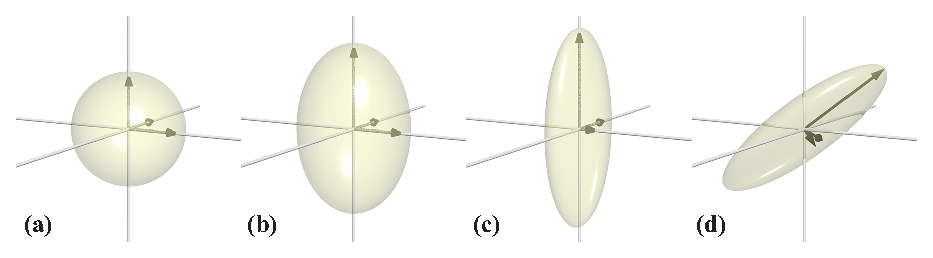
\includegraphics[width=0.98\textwidth]{tensorellipsoid}
\end{messagebox}








